\ch{Introduction}{einleitung}

\sect{Background \& Motivation}{background}

Recent progress in artificial intelligence (AI) and robotics has driven a paradigm shift from deterministic, preprogrammed automation toward adaptive and context-aware autonomous systems. Traditional robotic control architectures rely on explicit task definitions and rigid interfaces, which constrain scalability, flexibility, and human accessibility in dynamic environments. As robots are increasingly deployed in research laboratories, manufacturing facilities, and collaborative workspaces, the need for intuitive and semantically aligned communication between humans and machines has become critical. Conventional programming approaches such as teach pendants or vendor-specific languages remain incomprehensible to non-experts. In contrast, recent advances in natural language processing (NLP) and large language models (LLMs) enable direct translation of human intent into structured, machine-interpretable actions, creating a new form of human-robot communication grounded in shared semantics rather than fixed syntax. This emerging integration of linguistic reasoning with robotic control provides the foundation for cognitive autonomy, where robotic agents can interpret instructions, plan tasks, and execute operations within self-driving environments.


\sect{Problem Statement \& Objectives}{problem}

The conventional human-robot communication pipeline still relies heavily on intermediaries such as operators or technicians, who translate natural-language (NL) intentions into structured machine instructions through graphical interfaces or vendor-specific control software. This multi-stage translation process introduces latency, cognitive overhead, and potential for misinterpretation, preventing direct information flow between human and robot cell, as illustrated in Figure 1.1.

\begin{figure}[H]
    \centering
    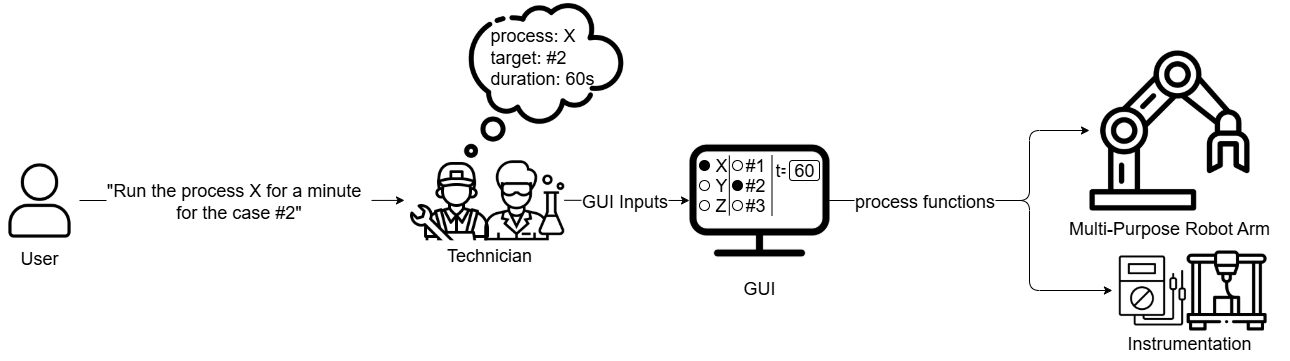
\includegraphics[width=1\linewidth]{Images/13.drawio.png}
    \caption{Conventional communication pipeline between user intent and robotic execution}
    \label{fig:labtechnicanoperator}
\end{figure}

This thesis investigates whether introducing an LLM as an intermediate reasoning layer can eliminate the dependency on manual translation in human-robot communication. The hypothesis is that such an LLM-based control layer can directly convert NL instructions into executable robotic commands, thereby reducing interpretation errors and improving consistency across collaborative robot cell such as Self-Driving Laboratories (SDLs). As can be seen in Figure~\ref{fig:llm_communication_framework}, the proposed architecture replaces the conventional multi-stage communication chain with a unified framework in which user intent is semantically processed and executed by the robotic system without intermediary reformulation.

\begin{figure}[H]
    \centering
    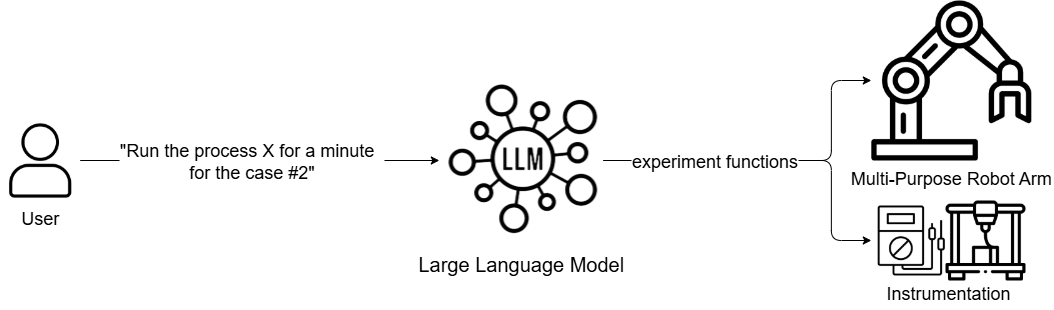
\includegraphics[width=0.85\linewidth]{Images/14.drawio.png}
    \caption{Proposed communication framework introducing an LLM-based intermediate layer for direct translation of user intent into robotic execution}
    \label{fig:llm_communication_framework}
\end{figure}

\sect{Scope \& Thesis Structure}{scope}

This thesis investigates the development and validation of a language-driven robotic control framework capable of autonomously interpreting and executing dedicated specialized tasks from NL instructions. The scope is limited to a single-robot, single-workstation SDL designed for electrochemical measurements, integrating a uFactory xArm6 manipulator and a programmable potentiostat. The work focuses on establishing a closed-loop control pipeline that connects human linguistic input, reasoning through a locally deployed LLM, using agentic frameworks, and deterministic tool execution within the SDL.

The thesis is structured as follows. \textbf{Chapter~2} reviews the state of the art in robotic programming, task planning, AI-driven autonomy, and language-based robot interaction, identifying the research gap motivating this study. \textbf{Chapter~3} introduces the conceptual and methodological framework of the proposed system, describing the multi-layer architecture linking the LLM agent, robot controller, and measurement instrumentation. \textbf{Chapter~4} details the practical implementation, including hardware integration, software realization, and the configuration of the LLM-based agent using the \textit{smolagents} framework. \textbf{Chapter~5} presents and analyses the experimental results obtained from simulated and real-user evaluations. \textbf{Chapter~6} discusses the findings with respect to robustness, scalability, and interaction quality, followed by \textbf{Chapter~7}, which outlines prospective improvements such as multi-agent orchestration, safety-aware reasoning, and extended multimodal grounding.